\chapter{Project Execution}
\label{chap:execution}

% \subsection{Generating the sample}
% \begin{itemize}
%       \item Discuss aligning hte article with returns
%       \begin{itemize}
%             \item Discuss private stocks and public stocks
%             \item Discuss non market days
%       \end{itemize}
%       \item Discuss pre processing the data
%       \item Discuss the kaggle sample
% \end{itemize}
In this section, we present the execution of the project, giving an overview of the dataset used, the configurations of hyperparameters and programming completed. The main idea of the project is to gather a dataset of headlines over a given time period and implement and analyse the algorithm presented by Ke et al. in their 2019 paper \cite{sestm}. Due to the difference in language used in headlines compared to that used in headlines, slightly different approaches were considered for some of the steps, but the theory behind the model remains unchanged.

\section{Project Components}
For this project, I opted to use Jupyter notebook as a base on which to implement the data processing, model training and validation, and portfolio formation. The modular nature of Jupyter, combined with Python's wide range of useful libraries facilitated the creation of this model. Creating each section as an independent cell allows for rigorous debugging and testing of each individual part, which would otherwise be extremely time consuming to test. The full notebook along with accompanying datasets can be found on GitHub \cite{github}.

\section{Dataset and Pre-Processing}
The dataset used for training and validation is available from Kaggle\footnote{\url{https://www.kaggle.com/datasets/miguelaenlle/massive-stock-news-analysis-db-for-nlpbacktests}} and is a collection of around 1.4 million headlines for 6000 stocks from 2009 to 2020. Each headline has the date published, and the ticker that the headline concerns. Some headlines have multiple tickers associated with them, but each ticker-headline combination is a unique entry in the dataset.

The first challenge is to align these headlines with the relevant three day returns, and this was achieved using the Yahoo Finance python library.\footnote{\url{https://pypi.org/project/yfinance/}} Once again, this relates to market close on day $t-2$ to close on day $t+1$ for a headline released on day $t$ (between 4pm on day $t-1$ to 4pm on day $t$). Some headlines are released on non-market days (such as weekends), and for these edge cases, the next available market day is selected as day $t$, and then the previous market day from this new day $t$ is defined as day $t-1$. Similarly, for market days where $t+1$ would fall on a non-market day, the next available market day is defined as day $t+1$. As many headline are released each day, computing the returns for each unique headline in this way would create significant redundancy, and therefore for each unique stock in the dataset, market data for the entire 11 year timespan is pulled in order to create a lookup table. Then, as opposed to calculating the stock values for each headline, if a headline is released on day $t$ relating to stock $s$, the open and close values can be retrieved via the key $(s,t)$. Finally, each headline is iterated through, assigning the appropriate market close values from the lookup table, and stored in json format for future usage. An example json entry is shown below in listing \ref{json} where `open' refers to market value of a ticker day $t-1$ and `close' refers to market value on day $t+1$.

\begin{lstlisting}[float={t},caption={Example JSON headline entry},label={json},language=c]
      {
            "headline": Barclays Maintains Equal-Weight on Agilent
            Technologies, Lowers Price Target to $76
            "date": 2020-03-26
            "ticker": A
            "mrkt_info": {
                  "open": 67.0
                  "close": 70.9100036621
            }
      }
\end{lstlisting}

\begin{lstlisting}[float={t},caption={Creating lookup table},label={lookup-table},language=Python]
day_t_data = {}
TOTAL_ARTS = len(stock_data)
for t in stock_data:
      # iterate through each ticker, and gather day t-1 (from_stock), 
      # day t and day t+1 (to_stock) data for ease of lookup
      #
      # to get day t: day_t_data[t][date]['day_t']
      ticker_date_data = {}
      start = min(stock_data[t].index)
      end = max(stock_data[t].index)
      curr_date = start
      while curr_date < end:
            day_t = curr_date
            while (not (day_t in stock_data[t].index) and day_t <= end):
                  day_t += dt.timedelta(days=1)
            from_stock = day_t - dt.timedelta(days=2)
            to_stock = day_t + dt.timedelta(days=1)
            while (not (from_stock in stock_data[t].index) and from_stock >= start):
                  from_stock -= dt.timedelta(days=1)
            while (not (to_stock in stock_data[t].index) and (to_stock <= end):
                  to_stock += dt.timedelta(days=1)
            if(from_stock > start and to_stock < end):
                  ticker_date_data[curr_date] = {
                        'day_t': day_t,
                        'from_stock': stock_data[t]['Close'][from_stock], 
                        'to_stock': stock_data[t]['Close'][to_stock]
                  }
            curr_date += dt.timedelta(days=1)
      day_t_data[t] = ticker_date_data
\end{lstlisting}

Note that some tickers do not have publicly available stock market information for the entire span of the sample. This is due to some companies being private for the duration, or turning private, meaning that their information is not accessible through standard means. Headlines aligned with these private tickers are removed from the sample, leaving around 1 million articles in the sample.

With the headlines aligned to the appropriate returns, the text data must be preprocessed to allow for successful and efficient semantic analysis. Taking the text content of each headline, the following transformations are applied, also detailed by figure \ref{fig:pre-processing-flow}:

\begin{figure}[!ht]
      \centering
      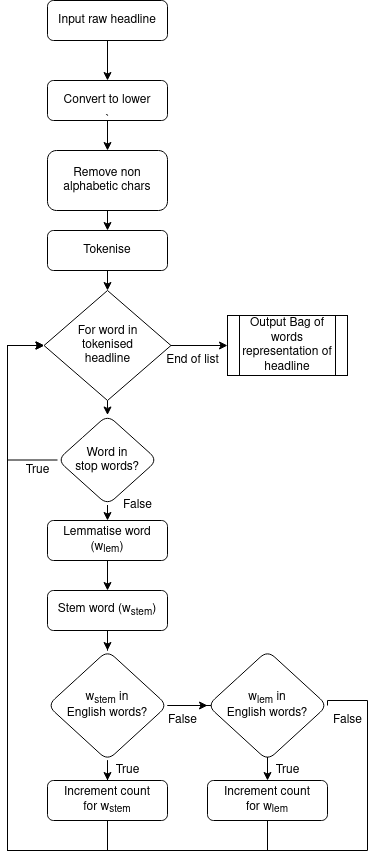
\includegraphics[scale=.6]{./pics/pre-processing-flowchart.png}
      \caption[Bag of words flowchart]{Flowchart showing conversion of raw headline into bag of words format}
      \label{fig:pre-processing-flow}
\end{figure}

\begin{itemize}
      \item Convert the headline to lower case. This is to ensure that different cases do not lead to multiple entries of the same word, differing only by letter captialisation.
      \item Remove non alphabetic characters
      \begin{itemize}
            \item Spaces are retained to allow for tokenisation
      \end{itemize}
      \item Tokenise the headline (convert to list of words)
      \item Remove non-English words \footnote{The list of English words is available from item 106 from \url{https://www.nltk.org/nltk_data/}}
      \item Remove stop words. \footnote{The list of stopwords used is from item 86 from \url{https://www.nltk.org/nltk_data/}} Stop words are a term used in NLP to describe very commonly used words that are unimportant (such as `and' or `the'). They serve only as noise and are removed to allow focus on more important news.
      \item Lemmatise each word (for example converting `mice' to `mouse' or `skis' to `ski') \footnote{The lemmatisation process uses WordNet (item 106) from \url{https://www.nltk.org/nltk_data/}}
      \item Stem each word (for example, `regional' to `region').\footnote{The stemming process uses Snowball stemmer from wordnet from \url{https://www.nltk.org/nltk_data/}} Note that as stemming aims to create the most general stem of a word, it sometimes leaves a word that is not English (such as `easily' to `easili'). For this reason, if the stemmed word is not in the list of English words, but the lemmatized word is, then this word is not stemmed.
      \item Convert to bag of words (BOW) representation (list of unique words with associated word counts for a given headline)
\end{itemize}

By utilising stemming where appropriate (i.e. when the stemmed word is included in the list of English words), we ensure that the resulting bag of words most closely resembles the original headline, while also grouping words that are similar by root. This helps to keep sentment consistent, as the root of a word is likely to be what holds sentiment, rather than the form it is used in. Another complication is the part of speech according to which a word is lemmatised. For example, the word `trying' is both a noun and a verb, depending on context (e.g. `a \textit{trying} quarter' versus `I was \textit{trying} really hard'). The lemmatisation of this word in the context of a noun is `trying', in verb context is `try' and the stem is `tri'. By default, the Wordnet Lemmatizer assumes the input is a noun, and I decided to do the same, at the potential risk of misclassifying a word. However, the shortcomings of treating each word as a noun are often covered by the stemming of the word, therefore using the two in conjunction gives the most accurate root of a word.


\section{Training the Model}
\label{sec:training-model}
Using the BOW representation of each of the headlines, the data is able to be processed according to the algorithm outlined by Ke et al. In the spirit of the original paper, the dataset is divided up into 17 three year training and validation windows, where two years are used for training a model, and the final year is used for validation purposes. More concretely, the training sample begins in 2010-01-01 and ends on 2017-12-31, the validation sample begins in 2012-01-01 and ends in 2018-12-31, leaving articles between 2019-01-01 and 2020-06-08 as an out of sample dataset used for testing the robustness of the model. All the computation is completed on this window, and then it is moved forward four months and repeated in a rolling window method.

\begin{table}[t]
\centering
\begin{tabular}{c>{\rowmac}c>{\rowmac}c>{\rowmac}c>{\rowmac}c>{\rowmac}c>{\rowmac}c>{\rowmac}c<{\clearrow}}
\toprule
Window start date & $|S|/2$ & $\alpha_+$ & $\alpha_-$ & $\kappa$ & $\lambda$ & Minimum error & Avg Min Error\\
\midrule
2010-1-1 & 100 & 0.0529 & 0.0487 & 92 & 5 & 20402.2 & 0.24727\\
2010-5-1 & 100 & 0.0405 & 0.0384 & 94 & 5 & 20714.66 & 0.24926\\
2010-9-1 & 25 & 0.1116 & 0.1043 & 92 & 5 & 20426.81 & 0.24675\\
2011-1-1 & 25 & 0.1023 & 0.1064 & 92 & 1 & 19963.67 & 0.24574\\
2011-5-1 & 50 & 0.1002 & 0.0921 & 90 & 5 & 19075.08 & 0.24598\\
2011-9-1 & 100 & 0.0425 & 0.0404 & 94 & 5 & 19255.78 & 0.24653\\
2012-1-1 & 100 & 0.0754 & 0.0744 & 88 & 5 & 20474.7 & 0.24744\\
2012-5-1 & 100 & 0.051 & 0.0489 & 92 & 10 & 21839.81 & 0.24961\\
2012-9-1 & 100 & 0.0536 & 0.0473 & 92 & 10 & 22243.55 & 0.24931\\
2013-1-1 & 50 & 0.0536 & 0.0672 & 94 & 5 & 21546.5 & 0.24702\\
\setrow{\bfseries}*2013-5-1 & 100 & 0.084 & 0.0913 & 86 & 5 & 22095.56 & 0.24552\\
2013-9-1 & 100 & 0.0688 & 0.076 & 88 & 10 & 23415.73 & 0.24885\\
2014-1-1 & 100 & 0.0395 & 0.0375 & 94 & 5 & 24819.11 & 0.24818\\
2014-5-1 & 100 & 0.0823 & 0.0954 & 86 & 5 & 24060.98 & 0.24652\\
2014-9-1 & 100 & 0.0392 & 0.0412 & 94 & 5 & 23536.73 & 0.24904\\
2015-1-1 & 100 & 0.0778 & 0.0898 & 86 & 5 & 22801.46 & 0.24805\\
2015-5-1 & 100 & 0.0471 & 0.0571 & 92 & 5 & 23642.32 & 0.24871\\
2015-9-1 & 100 & 0.0603 & 0.0734 & 90 & 5 & 26361.23 & 0.24772\\
2016-1-1 & 100 & 0.0478 & 0.0518 & 92 & 5 & 29950.54 & 0.24818\\
\bottomrule
\end{tabular}
\caption[Model configurations]{Best configuration and error for each window. Smallest error window highlighted in \textbf{bold}}
\label{min-error-train}
\end{table}

\begin{lstlisting}[float={!htb},caption={Calculating list of sentiment words},label={lst:calc-sentiment},language=Python]
kappa_configs   = [86, 88, 90, 92, 94]
alpha_configs   = [25,50,100]
# fraction of positively tagged training articles
train_pi = sum(sgn_i > 0 for sgn_i in train_sgn)/len(train_sgn)
for alpha in alpha_configs:
      for KAPPA in kappa_configs:
      #TRAINING
      kappa_percentile = np.percentile(np.array(list(total_j.values())),KAPPA)
      # return the nth percentile of all appearances for KAPPA

      #calculate alpha vals
      ALPHA_PLUS  = train_pi/2
      ALPHA_MINUS = train_pi/2
      delta_plus  = train_pi/4
      delta_minus  = train_pi/4
      # set limit on max iterations
      delta_limit = 0.0001
      
      while(delta_plus > delta_limit):
            no_pos_words = len([w for w in total_j if f[w] >= train_pi + ALPHA_PLUS and total_j[w] >= kappa_percentile])
            if no_pos_words == alpha:
                  # alpha plus found
                  delta_plus = 0
            elif (no_pos_words > alpha):
                  ALPHA_PLUS += delta_plus
                  delta_plus /= 2
            else:
                  ALPHA_PLUS -= delta_plus
                  delta_plus /= 2
      while(delta_minus > delta_limit):
            no_neg_words = len([w for w in total_j if f[w] <= train_pi - ALPHA_MINUS and total_j[w] >= kappa_percentile])
            if no_neg_words == alpha:
                  # alpha minus found
                  delta_minus = 0
            elif (no_neg_words > alpha):
                  ALPHA_MINUS += delta_minus
                  delta_minus /= 2
            else:
                  ALPHA_MINUS -= delta_minus
                  delta_minus /= 2
      sentiment_words = [w for w in total_j if ((f[w] >= train_pi + ALPHA_PLUS or f[w] <= train_pi - ALPHA_MINUS) and total_j[w] >= kappa_percentile)]
\end{lstlisting}

The training section employs the screening (section \ref{screen-sentiment}) and learning (section \ref{learn-sentiment}) steps, while the validation is the application of the scoring new headlines (section \ref{new-headlines}) step. The validation section is used to consider the hyperparameters ($\alpha_+, \alpha_-, \kappa, \lambda$), and these are evaluated according to a fixed number of possibilities. $\alpha_\pm$ is calculated such that $S$ has either 25, 50, or 100 words of each sentiment (i.e. for the selection of $\alpha = 25$, $|S| = 50$). This is calculated via binary search, assuming $\alpha_\pm = 0.25$ at first. If the resulting set of words is larger than the selected configuration, then $\alpha$ must be larger than the current value, as the larger $\alpha$ is, the fewer words satisfy the condition. Similarly, the inverse for the case where the set of words contains fewer words than desired. $\kappa$ is selected to be the 86, 88, 90, 92 or 94th percentiles of word counts. Note that the $\kappa$ restraint is applied first such that a word is not selected via the $\alpha$ constraint that must then be removed due to the $\kappa$ constraint, leaving $S$ with fewer words than desired. Combining both the calculated $\alpha_\pm$ values and the calculated $\kappa$ value, the list of sentiment words for the training window is compiled, illustrated in listing \ref{lst:calc-sentiment}. Finally, $\lambda$ is selected to be either 1, 5, or 10, for a total of 45 configurations.

Each of these 45 configurations is iterated through for each window, and the $\ell^1$ error is calculated for each, before selecting the setup with minimum error (as this is our loss function). $\ell^1$ error in this case is simply:


\begin{equation}
\sum_{i=1}^{n}|\widehat{p_i} - p_i|
\end{equation}

\noindent
where $\widehat{p_i}$ is the estimated sentiment and $p_i$ is the standardised return rank of article $i$ in the validation set. The loss function of $\ell^1$-norm error was selected for its robustness. The entire process of training and validation takes a considerable length of time and therefore some time was spent optimising the code. A complete list of optimisations can be found in appendix (REFERENCE) %TODO: add optimisation list and reference it


Table \ref{min-error-train} details the results of the completed rolling window training. Due to the nature of news, some validation sets are larger than others, leading to skewed summed $\ell^1$-norm error. To accommodate for this variation is sample size, the error is taken as an average over all headlines in the sample. Window 2011-1-1 has the smallest minimum error, but also has the smallest validation sample size and after controlling for this factor, window 2013-5-1 is has slightly lower error, meaning this is the optimum window.

\subsection{Bigram training}
Naturally, the order in which words appear in a headline can have a profound impact on the sentiment of a word. This can be captured by training the model on \textit{bigrams}, which are sequences of two words, rather than single words alone. This can then be combined with the lexicon of unigrams to provide a clearer insight into the true sentiment of a headline based on the words used.


\begin{lstlisting}[float={!htb},caption={Calculating list of sentiment words},label={lst:bigram-formation},language=Python]
KAPPA_BIGRAM = 90
kappa_percentile_bigram = np.percentile(np.array(list(total_j.values())),KAPPA_BIGRAM)
# return the nth percentile of all appearances for KAPPA_BIGRAM
bigrams_to_remove = []
mutual_info = {}
for w in total_j_bigram:
      component_words = w.split()
      if not (total_j[component_words[0]] >= kappa_percentile_bigram and total_j[component_words[1]] >= kappa_percentile_bigram):
      bigrams_to_remove.append(w)
      else:
      mutual_info[w] = total_j_bigram[w] / (total_j[component_words[0]] * total_j[component_words[1]])
mutual_info_percentile = np.percentile(np.array(list(mutual_info.values())),95)
bigrams_to_remove.extend([w for w in mutual_info if mutual_info[w] <= mutual_info_percentile])
for b in bigrams_to_remove:
      pos_j_bigram.pop(b)
      total_j_bigram.pop(b)
      f_bigram.pop(b)
\end{lstlisting}

The algorithm naturally lends itself to training with bigrams and little is needed in the way of adjustment, as the bigrams are treated the same way as words. The only slight difference is the way that bigrams are filtered out. Due to the nature of bigrams, they will be, on average, far less frequent than unigrams, simply because of the increased number of possibilities. For this reason, centain measures are taken to ensure that only meaningful bigrams are considered. For each window, all articles are divided into bigrams in the same way that the BOW representations are created. Stopwords are not considered for potential bigrams, and as such if two words are separated by a stop word, the resulting bigram would be as if the stop word were absent (e.g. `chalk and cheese' would create the bigram `chalk cheese'). Then, bigrams are removed if either component word is not common (below 85th quantile of word counts). Among the remaining phrases, only those bigrams with mutual information ranking in the top 5\% are retained. Mutual information score is calculated as the ratio of the frequency of the bigram divided by the product of the frequency of the component words. The percentile chosen here is slightly higher than the 1\% used by the original paper, as the dataset contained articles, meaning there are far more bigrams than in the dataset used here. For this reason, I chose to consider a higher number of bigrams to ensure completeness. After this filtering step, the rest of the training continues as before. The preparation for bigrams is shown in listing \ref{lst:bigram-formation}.

\section{Out of Sample Testing}
Using the optimally trained model (shown in table \ref{min-error-train}), the articles not used in either training or validation samples are then used to determine the strength of the model. Each market day $t$, the headlines released from 9 a.m. on day $t-1$ to 9 a.m. on day $t$ are selected and ranked $p$ value calculated from the scoring step (\ref{new-headlines}). Each ticker in the sample is then ranked according to sentiment of related headlines for that day. If a ticker has multiple headlines, the average sentiment from all related headlines is taken for the firm. From this, a portfolio is created, where the top 50 sentiment stocks are bought, and the lowest 50 sentiment stocks are shorted.

Some constraints are placed on the stocks that can be chosen, to ensure that stocks are not bought when they have negative sentiment. For a stock to be bought, it must have $\widehat p_i < 0.5$, and the inverse for a stock to be sold. On the occasion where there are not 50 stocks with positive sentiment, this is to avoid the portfolio purchasing slightly negative stocks, and therefore less than 50 stocks are used in this instance.
%TODO: say why 9 to 9 and not 9.30 (which is market open)


% \section{What to do}


% \noindent
% This chapter is intended to describe what you did: the goal is to explain
% the main activity or activities, of any type, which constituted your work 
% during the project.  The content is highly topic-specific, but for many 
% projects it will make sense to split the chapter into two sections: one 
% will discuss the design of something (e.g., some hardware or software, or 
% an algorithm, or experiment), including any rationale or decisions made, 
% and the other will discuss how this design was realised via some form of 
% implementation.  

% This is, of course, far from ideal for {\em many} project topics.  Some
% situations which clearly require a different approach include:

% \begin{itemize}
% \item In a project where asymptotic analysis of some algorithm is the goal,
%       there is no real ``design and implementation'' in a traditional sense
%       even though the activity of analysis is clearly within the remit of
%       this chapter.
% \item In a project where analysis of some results is as major, or a more
%       major goal than the implementation that produced them, it might be
%       sensible to merge this chapter with the next one: the main activity 
%       is such that discussion of the results cannot be viewed separately.
% \end{itemize}

% \noindent
% Note that it is common to include evidence of ``best practice'' project 
% management (e.g., use of version control, choice of programming language 
% and so on).  Rather than simply a rote list, make sure any such content 
% is useful and/or informative in some way: for example, if there was a 
% decision to be made then explain the trade-offs and implications 
% involved.

% \section{Example Section}

% This is an example section; 
% the following content is auto-generated dummy text.

% \subsection{Example Sub-section}

% \begin{figure}[t]
% \centering
% foo
% \caption{This is an example figure.}
% \label{fig}
% \end{figure}

% \begin{table}[t]
% \centering
% \begin{tabular}{|cc|c|}
% \hline
% foo      & bar      & baz      \\
% \hline
% $0     $ & $0     $ & $0     $ \\
% $1     $ & $1     $ & $1     $ \\
% $\vdots$ & $\vdots$ & $\vdots$ \\
% $9     $ & $9     $ & $9     $ \\
% \hline
% \end{tabular}
% \caption{This is an example table.}
% \label{tab}
% \end{table}

% \begin{algorithm}[t]
% \For{$i=0$ {\bf upto} $n$}{
%   $t_i \leftarrow 0$\;
% }
% \caption{This is an example algorithm.}
% \label{alg}
% \end{algorithm}

% \begin{lstlisting}[float={t},caption={This is an example listing.},label={lst},language=C]
% for( i = 0; i < n; i++ ) {
%   t[ i ] = 0;
% }
% \end{lstlisting}

% This is an example sub-section;
% the following content is auto-generated dummy text.
% Notice the examples in Figure~\ref{fig}, Table~\ref{tab}, Algorithm~\ref{alg}
% and Listing~\ref{lst}.

% \subsubsection{Example Sub-sub-section}

% This is an example sub-sub-section;
% the following content is auto-generated dummy text.

% \paragraph{Example paragraph.}

% This is an example paragraph; note the trailing full-stop in the title,
% which is intended to ensure it does not run into the text.

% -----------------------------------------------------------------------------